% Copyright (c) 2022 by Lars Spreng
% This work is licensed under the Creative Commons Attribution 4.0 International License.

\documentclass[
11pt,notheorems,hyperref={pdfauthor=whatever}
]{beamer}

\usepackage{kotex}
\input{loadslides.tex}

\usepackage{fontspec}
\IfFileExists{/Users/seojunha/Library/Fonts/NotoSansCJKkr-Regular.otf}{%
  \setmainhangulfont[
    Path=/Users/seojunha/Library/Fonts/,
    BoldFont=NotoSansCJKkr-Bold.otf
  ]{NotoSansCJKkr-Regular.otf}
  \setsanshangulfont[
    Path=/Users/seojunha/Library/Fonts/,
    BoldFont=NotoSansCJKkr-Bold.otf
  ]{NotoSansCJKkr-Regular.otf}
  \setmonohangulfont[
    Path=/Users/seojunha/Library/Fonts/,
    BoldFont=NotoSansCJKkr-Bold.otf
  ]{NotoSansCJKkr-Regular.otf}
}{%
  \IfFontExistsTF{Noto Sans CJK KR}{%
    \setmainhangulfont{Noto Sans CJK KR}
    \setsanshangulfont{Noto Sans CJK KR}
    \setmonohangulfont{Noto Sans CJK KR}
  }{%
    \IfFontExistsTF{NanumGothic}{%
      \setmainhangulfont{NanumGothic}
      \setsanshangulfont{NanumGothic}
      \setmonohangulfont{NanumGothic}
    }{}%
  }%
}
\renewcommand{\familydefault}{\sfdefault}

\usepackage{tikz}
\usetikzlibrary{arrows.meta, positioning, fit, backgrounds, calc, shapes.geometric}
\usepackage{booktabs}
\usepackage{array}

\definecolor{TextGray}{HTML}{333333}
\definecolor{DeepBlue}{HTML}{08457E}
\definecolor{SoftBlue}{HTML}{EAF0F8}
\definecolor{LineGray}{HTML}{B8B8B8}
\definecolor{WarnRed}{HTML}{B3261E}
\definecolor{GoodGreen}{HTML}{237A4B}
\definecolor{SoftGreen}{HTML}{EAF6EF}
\definecolor{SoftRed}{HTML}{FBEAEA}
\definecolor{SoftYellow}{HTML}{FFF4D8}

\addtobeamertemplate{frametitle}{}{\vspace{-0.5em}}
\setbeamerfont{title}{size=\LARGE,series=\bfseries}
\setbeamerfont{subtitle}{size=\normalsize}
\setbeamerfont{frametitle}{series=\bfseries}

\tikzset{
  nodebox/.style={draw=LineGray, rounded corners=2pt, fill=white, align=center, minimum height=0.82cm, inner sep=5pt, font=\small},
  bluebox/.style={draw=DeepBlue, very thick, rounded corners=2pt, fill=SoftBlue, align=center, minimum height=0.82cm, inner sep=5pt, font=\small\bfseries},
  redbox/.style={draw=WarnRed, very thick, rounded corners=2pt, fill=SoftRed, align=center, minimum height=0.82cm, inner sep=5pt, font=\small\bfseries},
  greenbox/.style={draw=GoodGreen, very thick, rounded corners=2pt, fill=SoftGreen, align=center, minimum height=0.82cm, inner sep=5pt, font=\small\bfseries},
  yellowbox/.style={draw=orange!70!black, very thick, rounded corners=2pt, fill=SoftYellow, align=center, minimum height=0.82cm, inner sep=5pt, font=\small\bfseries},
  arrow/.style={-{Latex[length=2.6mm]}, thick, draw=DeepBlue},
  grayarrow/.style={-{Latex[length=2.4mm]}, thick, draw=LineGray},
  badarrow/.style={-{Latex[length=2.4mm]}, thick, draw=WarnRed},
  goodarrow/.style={-{Latex[length=2.4mm]}, thick, draw=GoodGreen}
}

\newcommand{\smallgray}[1]{{\scriptsize\textcolor{gray!75}{#1}}}
\newcommand{\smallred}[1]{{\scriptsize\textcolor{WarnRed}{#1}}}
\newcommand{\smallblue}[1]{{\scriptsize\textcolor{DeepBlue}{#1}}}
\newcommand{\term}[1]{\textbf{\textcolor{DeepBlue}{#1}}}

\title[]{Why Reasoning Fails to Plan}
\subtitle{A Planning-Centric Analysis of Long-Horizon Decision Making in LLM Agents}
\author[]{하서준}
\institute{DGIST}
\date{2026년 6월 4일}

\begin{document}

{
\setbeamertemplate{footline}{}
\begin{frame}
  \titlepage
  \vspace{-0.8em}
  \begin{center}
  \scriptsize
  Reasoning \(\neq\) Planning \(\cdot\) Lookahead \(\cdot\) MCTS \(\cdot\) FLARE
  \end{center}
\end{frame}
}
\addtocounter{framenumber}{-1}

\begin{frame}[plain]
\centering
\vspace{0.22\textheight}
{\Large\bfseries Why Reasoning Fails to Plan:\\A Planning-Centric Analysis of\\Long-Horizon Decision Making in LLM Agents}
\vspace{1.2em}

{\small Zehong Wang et al.}\\
{\scriptsize Preprint 2026}
\end{frame}

\begin{frame}{논문이 제기한 문제점}
\vspace{0.15em}
\begin{alertblock}{문제점}
\small
LLM reasoning은 step-wise local score가 높은 action을 고르는 경향이 있어, 긴 horizon에서는 초반 myopic choice가 회복하기 어려운 failure로 증폭된다.
\end{alertblock}

\vspace{0.15em}
\begin{block}{논문의 해결 방향}
\small
Reasoning을 더 잘하게 만드는 것이 아니라, \textbf{미래 결과가 현재 action value로 되돌아오는 planning rule}을 넣어야 한다.
\end{block}

\vspace{0.25em}
\begin{center}
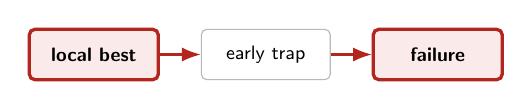
\begin{tikzpicture}[scale=0.78, transform shape]
\node[redbox, minimum width=2.1cm] (local) at (0,0) {local best};
\node[nodebox, minimum width=2.1cm] (trap) at (2.8,0) {early trap};
\node[redbox, minimum width=2.1cm] (fail) at (5.6,0) {failure};
\draw[badarrow] (local) -- (trap);
\draw[badarrow] (trap) -- (fail);
\end{tikzpicture}
\end{center}

\vspace{-0.1em}
\begin{block}{Coherent planning의 3가지 필수 요건}
\scriptsize
\begin{tabular}{@{}p{0.30\textwidth}p{0.31\textwidth}p{0.31\textwidth}@{}}
\textbf{1. Future evaluation} &
\textbf{2. Value propagation} &
\textbf{3. Limited commitment} \\
현재 action이 만드는 미래 trajectory를 평가 &
미래 outcome을 앞 action의 \(Q\)로 되돌려 반영 &
전체 plan에 commit하지 않고 한 step 실행 후 replanning \\
\end{tabular}
\end{block}
\end{frame}

\begin{frame}{FLARE Framework Overview}
\vspace{-0.1em}
\begin{center}
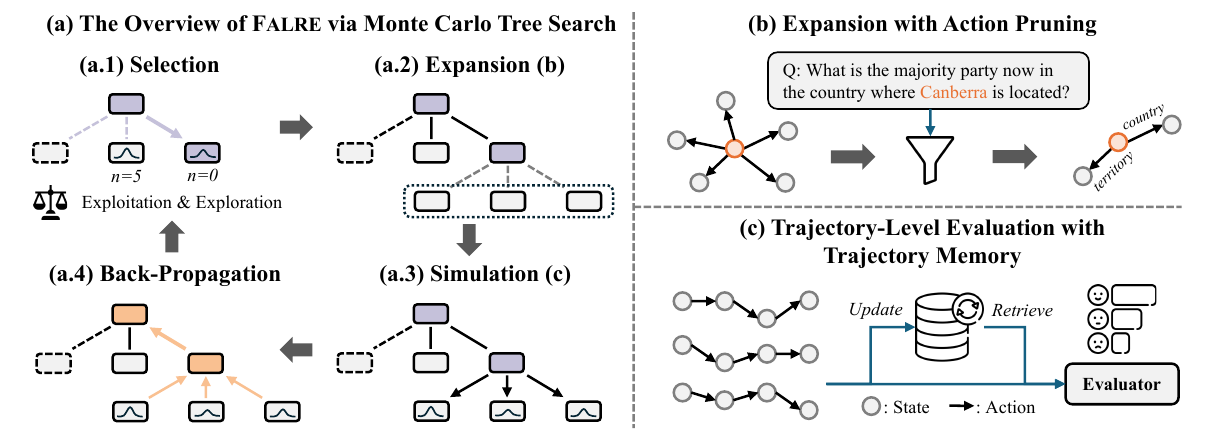
\includegraphics[width=0.98\textwidth]{figures/wrfp_fig5_flare_overview.png}
\end{center}
\vspace{-0.35em}
\begin{block}{핵심 구조}
\scriptsize
\begin{tabular}{@{}p{0.23\textwidth}p{0.23\textwidth}p{0.23\textwidth}p{0.23\textwidth}@{}}
\textbf{Selection} &
\textbf{Expansion} &
\textbf{Simulation} &
\textbf{Back-propagation} \\
UCB로 promising branch 선택 &
action pruning으로 후보 확장 &
후보 trajectory를 미리 rollout &
trajectory value를 앞 action의 \(Q\)에 반영 \\
\end{tabular}

\vspace{0.3em}
현재 state를 root로 두고 이 과정을 반복한 뒤, \textbf{가장 높은 value의 action 하나만 실행}하고 다음 state에서 다시 계획한다.
\end{block}
\end{frame}

\begin{frame}{방법: FLARE는 MCTS로 미래를 보고 한 step만 선택}
\vspace{0.1em}
\begin{block}{Selection rule: 논문 수식 (7)}
\centering
\Large
\[
a_t=\arg\max_{a\in A(s_t)}
\left[
\underbrace{Q(s_t,a)}_{\substack{\text{\scriptsize 미래 rollout 결과가}\\[-0.15em]\text{\scriptsize 누적된 action value}}}
+
\underbrace{c}_{\substack{\text{\scriptsize 탐색 강도}\\[-0.15em]\text{\scriptsize 조절}}}
\underbrace{\sqrt{\frac{\log N(s_t)}{N(s_t,a)+1}}}_{\substack{\text{\scriptsize 덜 가본 action}\\[-0.15em]\text{\scriptsize 선택 보너스}}}
\right]
\]
\end{block}

\vspace{0.5em}
\begin{center}
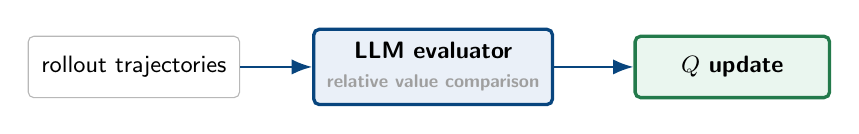
\begin{tikzpicture}[scale=0.95, transform shape]
\node[nodebox, minimum width=2.5cm] (rollout) at (0,0) {rollout trajectories};
\node[bluebox, minimum width=3.1cm] (eval) at (4,0) {LLM evaluator\\\smallgray{relative value comparison}};
\node[greenbox, minimum width=2.6cm] (q) at (8,0) {\(Q\) update};
\draw[arrow] (rollout) -- (eval);
\draw[arrow] (eval) -- (q);
\end{tikzpicture}
\end{center}

\vspace{0.25em}
\begin{block}{LLM이 하는 일}
\small
각 rollout trajectory를 독립적인 step 점수로 보지 않고, \textbf{trajectory 간 상대 가치}를 비교해서 return estimate를 만든다. 이 값이 backpropagation으로 앞 action의 \(Q(s_t,a)\)에 반영된다.
\end{block}
\end{frame}

\begin{frame}{진단 Figure: step-wise decision은 왜 무너지는가}
\vspace{-0.2em}
\begin{columns}[T,onlytextwidth]
\begin{column}{0.55\textwidth}
\centering
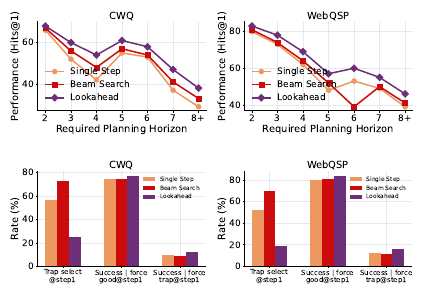
\includegraphics[width=0.94\textwidth]{figures/result_graph_only.png}

\vspace{0.25em}
\begin{block}{아래 bar plot 지표}
\scriptsize
\begin{itemize}
  \item \textbf{Trap select@step1}: 첫 action을 자유롭게 고를 때 trap을 선택한 비율
  \item \textbf{Success | force good@step1}: 첫 action을 좋은 action으로 고정했을 때 성공률
  \item \textbf{Success | force trap@step1}: 첫 action을 trap으로 고정했을 때 성공률
\end{itemize}
\end{block}
\end{column}
\begin{column}{0.42\textwidth}
\begin{block}{비교한 decision rule}
\small
\textbf{Single-step}\\
{\scriptsize\textcolor{TextGray}{현재 step의 local score가 가장 높은 action 하나만 선택}}

\vspace{0.6em}
\textbf{Beam search}\\
{\scriptsize\textcolor{TextGray}{single-step 선택을 하나만 남기지 않고, 좋아 보이는 후보 path \(k\)개를 동시에 탐색}}

\vspace{0.6em}
\textbf{Lookahead}\\
{\scriptsize\textcolor{TextGray}{후보 action마다 짧은 미래 rollout을 보고 cumulative return으로 선택}}
\end{block}

\vspace{0.25em}
\begin{alertblock}{Figure의 메시지}
\small
Single-step/beam은 horizon이 길어질수록 early trap에 commit하고 회복이 어렵다. Lookahead는 미래 결과를 보므로 trap 선택과 error accumulation을 줄인다.
\end{alertblock}
\end{column}
\end{columns}
\end{frame}

\begin{frame}{결과: accuracy뿐 아니라 planning behavior가 바뀜}
\vspace{0.05em}
\begin{columns}[T,onlytextwidth]
\begin{column}{0.48\textwidth}
\centering
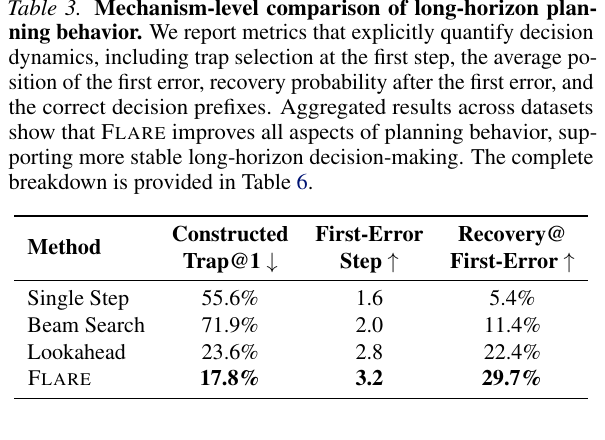
\includegraphics[width=\textwidth]{figures/wrfp_table3_mechanism.png}
\end{column}
\begin{column}{0.48\textwidth}
\begin{block}{핵심 지표}
\small
\begin{itemize}
  \item \term{Trap@1}: 첫 선택에서 ``당장은 좋아 보이지만 나중에 막히는 action''을 고른 비율
  \item \term{First-Error}: optimal path에서 처음 벗어나는 평균 step
  \item \term{Recovery}: 한 번 틀어진 뒤에도 다시 정답에 도달한 비율
\end{itemize}
\end{block}
\end{column}
\end{columns}

\vspace{0.25em}
\begin{alertblock}{결과 해석}
\small
Single-step과 beam search는 local score에 묶여 초반 trap을 자주 선택하고, 한 번 벗어나면 거의 회복하지 못한다. Lookahead는 짧은 미래 평가로 trap을 줄이지만 효과가 제한적이다. FLARE는 trajectory outcome을 \(Q\)로 되돌려 반영하므로 \textbf{trap을 가장 적게 고르고, 오류를 더 늦추며, recovery도 가장 높다}.
\end{alertblock}
\end{frame}

\begin{frame}{그래서 어떻게?}
\vspace{0.25em}
\begin{columns}[T,onlytextwidth]
\begin{column}{0.48\textwidth}
\begin{block}{1. Confidence agent 학습}
\small
다양한 evidence subset을 입력으로 주고, 그 subset만 보고 진단 confidence를 잘 내도록 학습한다.

\vspace{0.45em}
\smallgray{목표: ``현재까지 모은 정보로 얼마나 확신할 수 있는가''를 안정적으로 추정}
\end{block}
\end{column}
\begin{column}{0.48\textwidth}
\begin{block}{2. Planner 학습}
\small
confidence agent는 고정하고, planner가 후보 action을 lookahead해본 뒤 어떤 검사를 할지 선택하도록 학습한다.

\vspace{0.45em}
\smallgray{목표: 당장 그럴듯한 검사가 아니라, 이후 confidence를 가장 잘 개선하는 검사 선택}
\end{block}
\end{column}
\end{columns}

\vspace{0.65em}
\begin{center}
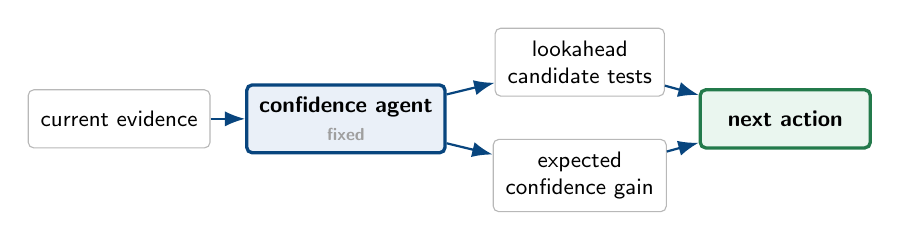
\begin{tikzpicture}[scale=0.9, transform shape]
\node[nodebox, minimum width=2.3cm] (state) at (0,0) {current evidence};
\node[bluebox, minimum width=2.5cm] (conf) at (3.2,0) {confidence agent\\\smallgray{fixed}};
\node[nodebox, minimum width=2.3cm] (roll) at (6.5,0.8) {lookahead\\candidate tests};
\node[greenbox, minimum width=2.4cm] (act) at (9.4,0) {next action};
\node[nodebox, minimum width=2.3cm] (update) at (6.5,-0.8) {expected\\confidence gain};
\draw[arrow] (state) -- (conf);
\draw[arrow] (conf) -- (roll);
\draw[arrow] (roll) -- (act);
\draw[arrow] (conf) -- (update);
\draw[arrow] (update) -- (act);
\end{tikzpicture}
\end{center}

\vspace{0.25em}
\begin{alertblock}{핵심}
\small
진단 모델을 매번 바꾸기보다, \textbf{confidence를 평가하는 agent}와 \textbf{정보 획득을 계획하는 planner}를 분리한다.
\end{alertblock}
\end{frame}

\end{document}
